% Provenance (never printed): see sources/outline_sources.md (Year 2: the Himalaya and Tibet;
% the Andes; crustal thickening and plateaus). Himalayan units, thrusts and rates after Lave
% and Avouac (2000), Ader et al. (2012), Cattin et al. (2001), Dong et al. (2026, STDS);
% Asian extrusion after Jiao et al. (2023); Tibetan rifts after Wang et al. (2021); Central
% Andes after Gerbault et al. (2005); flat slabs after Gauthier et al. (2024). Relief from
% ETOPO1 (figdata/bachelor-2/plateaus.py); plate velocities from NNR-MORVEL56 (Book 2 ledger
% row nnr56:poles). Exercise and problem values in the Book 4 scratch calculator
% calc/ch14.py.
\chapter{Botsingsgordels en Andesgordels vergeleken}\label{ch:b2:himalaya-andes}

Twee plateaus op Aarde liggen over honderden kilometers meer dan vier kilometer hoog.
Tibet werd opgeheven waar India tegen Azië botste, twee continenten die elkaar ontmoetten nadat de oceaan ertussen
verdwenen was. De Altiplano werd opgeheven waar een oceanische plaat, de Nazcaplaat, nog steeds
onder Zuid-Amerika schuift, zonder dat er enig continent aankomt. Twee verschillende motoren bouwden twee
soortgelijke landvormen. Dit hoofdstuk neemt de twee gordels uit elkaar, meet hoe dik hun korst
is geworden en waarom, en vraagt wat hen belet nog hoger te groeien.
% ledger: lave00:setting, gerbault05:andes, data:b4-etopo-tibet, data:b4-etopo-andes

\begin{recall}
\textbf{Uit Boek~2}: continentale botsing en de sutuur; de noordwaartse
drift van India, de vertraging ervan en de omstreden ouderdom van de botsing; het Tibetaans Plateau ongeveer
\qty{4600}{m} hoog boven een korst van ongeveer \qty{70}{km} dik. \textbf{Uit Boek~3}:
Airy-isostasie en de Bouguer-plaat; actieve randen, de subducerende plaat, de vulkanische boog en
de afstand tussen boog en trog; plaatsnelheden uit hoeksnelheden; de wet van Byerlee; de
momentmagnitude. \textbf{Uit \cref{ch:b2:crustal-melting}}: \omterm{def:b2:crustal-melting:leucogranite}{leucogranieten} van de Himalaya.
\textbf{Uit \cref{ch:b2:alpine-orogen}}: \omterm{def:b2:alpine-orogen:orogen}{orogeen}, \omterm{def:b2:alpine-orogen:nappes}{dekblad}, \omterm{def:b2:alpine-orogen:decollement}{décollement}, dunhuidige en
\omterm{def:b2:alpine-orogen:skin}{dikhuidige tektoniek}, \omterm{def:b2:alpine-orogen:ftb}{plooi- en overschuivingsgordel}, \omterm{def:b2:alpine-orogen:foreland}{voorlandbekken}, \omterm{def:b2:alpine-orogen:balanced}{gebalanceerde doorsneden}.
\end{recall}

\begin{definition}[Botsingsorogeen; orogeen van Andestype]\label{def:b2:himalaya-andes:types}
Een \emph{botsingsorogeen}\index{botsingsorogeen} is een \omterm{def:b2:alpine-orogen:orogen}{orogeen} dat is opgebouwd door de convergentie van
twee continentale randen nadat de oceaan ertussen is verbruikt; zijn as is een sutuur.
Een \emph{orogeen van Andestype}\index{orogeen van Andestype} is een \omterm{def:b2:alpine-orogen:orogen}{orogeen} dat is opgebouwd op de bovenliggende
plaat van een subductiezone tussen oceaan en continent, terwijl de subductie eronder doorgaat; zijn as
is een vulkanische boog.
\end{definition}


\section{India tegen Azië}\label{sec:b2:himalaya-andes:himalaya}

India bereikte de zuidrand van Eurazië ongeveer 50 miljoen jaar geleden langs de
Indus--Tsangpo-sutuur, ook Indus--Yarlung-sutuur genoemd; de precieze datum staat nog ter discussie, zoals
Boek~2 liet zien. De convergentie stopte niet. Vandaag naderen India en Azië elkaar
met ongeveer \qty{40}{mm} per jaar; volgens de hoeksnelheden van het platenmodel NNR-MORVEL56
beweegt India met \qty{45}{mm} per jaar ten opzichte van Eurazië op \ang{28}~NB, \ang{85}~OL, in de richting
\ang{22} ten oosten van het noorden. Slechts een deel van die beweging wordt in de Himalaya opgevangen. Over Nepal
tonen GPS-stations dat India en Zuid-Tibet convergeren met $17.8 \pm \qty{0.5}{mm}$ per jaar in het
midden en oosten en $20.5 \pm \qty{1}{mm}$ per jaar in het westen: ongeveer de helft van het totaal. De rest
wordt over Tibet en de rest van Azië verdeeld.
% ledger: lave00:setting, najman21:collision-age, jiao23:extrusion, nnr56:poles, ader12:rates, ader12:mht
% values (plateaus.py): v_india_eurasia 44.99 mm/yr, azimuth 21.65

De kaarten hieronder tonen de twee gordels met dezelfde hoogtelijnen, en de stroken waarlangs dit
hoofdstuk ze doorsnijdt.

\begin{omfigure}
\centering
% ledger: data:b4-etopo-tibet, data:b4-etopo-andes
\begin{tikzpicture}
\begin{axis}[name=tib, scale only axis, width=8.0cm, height=4.8cm, xmin=75, xmax=100,
  ymin=25, ymax=40, xlabel={lengtegraad (\unit{\degree} OL)}, ylabel={breedtegraad (\unit{\degree} NB)},
  tick label style={font=\scriptsize}, label style={font=\small}, xtick={75,80,...,100},
  ytick={25,30,...,40}, title={\small Himalaya en Tibet}]
\addplot[omThm!35, line width=0.3pt] table[x=lon, y=lat] {figdata/out/bachelor-2-plateaus-tc2000.dat};
\addplot[omThm!90!black, line width=0.4pt] table[x=lon, y=lat] {figdata/out/bachelor-2-plateaus-tc4000.dat};
\draw[black, densely dashed, line width=0.9pt] (axis cs:86,25) rectangle (axis cs:90,40);
\node[font=\scriptsize, fill=white, fill opacity=0.85, text opacity=1, inner sep=1pt] at (axis cs:80,26.2) {Gangesvlakte};
\node[font=\scriptsize, fill=white, fill opacity=0.85, text opacity=1, inner sep=1pt] at (axis cs:94.5,33.5) {Tibetaans Plateau};
\node[font=\scriptsize, fill=white, fill opacity=0.85, text opacity=1, inner sep=1pt] at (axis cs:83,39.2) {Tarim};
\end{axis}
\begin{axis}[at={(tib.east)}, anchor=west, xshift=1.6cm, scale only axis, width=3.6cm,
  height=4.8cm, xmin=-75, xmax=-60, ymin=-30, ymax=-10,
  xlabel={lengtegraad (\unit{\degree})}, tick label style={font=\scriptsize},
  label style={font=\small}, xtick={-75,-70,-65,-60}, ytick={-30,-25,...,-10},
  title={\small Centrale Andes}]
\addplot[blue!60!black, line width=0.45pt] table[x=lon, y=lat] {figdata/out/bachelor-2-plateaus-ac0.dat};
\addplot[omThm!35, line width=0.3pt] table[x=lon, y=lat] {figdata/out/bachelor-2-plateaus-ac2000.dat};
\addplot[omThm!90!black, line width=0.4pt] table[x=lon, y=lat] {figdata/out/bachelor-2-plateaus-ac4000.dat};
\draw[black, densely dashed, line width=0.9pt] (axis cs:-75,-21) rectangle (axis cs:-60,-19);
\node[font=\scriptsize, fill=white, fill opacity=0.85, text opacity=1, inner sep=1pt] at (axis cs:-73,-25) {Stille Oceaan};
\end{axis}
\end{tikzpicture}
\par\smallskip{\small Reliëf van de twee gordels volgens ETOPO1, met een knoop om de \qty{0.1}{\degree}:
hoogtelijnen op \qty{2000}{m} (licht) en \qty{4000}{m} (donker), en de kustlijn op de
rechterkaart. Breedtegraden op de rechterkaart zijn negatief ten zuiden van de evenaar, lengtegraden negatief ten westen van
Greenwich. De gestreepte vakken zijn de stroken van de profielen verderop: \qtyrange{86}{90}{\degree} OL
over de Himalaya en Tibet, \qtyrange{19}{21}{\degree} ZB over de Centrale Andes.}
\end{omfigure}

\subsection{De eenheden en de overschuivingen}

Vanaf de Gangesvlakte naar het noorden doorkruist een doorsnede door de Himalaya een stapel overschuivingsplaten
die uit de noordrand van India zijn gesneden, gescheiden door breuken die over de hele lengte van de keten lopen.
\begin{itemize}
\item De \emph{Indo-Gangetische voordiepte} is het \omterm{def:b2:alpine-orogen:foreland}{voorlandbekken} van de Himalaya; ze vangt een deel van
het puin op dat van de keten erodeert.
\item De \emph{sub-Himalaya}, de Siwalikheuvels, bestaat uit de \omterm{def:b2:alpine-orogen:foreland}{molasse} van dat bekken,
kleistenen tot conglomeraten van Laat-Mioceen tot Pleistoceen, 3500 tot \qty{5500}{m} dik,
afgezet tussen 14 en \qty{1}{Ma}, daarna aan het front van de keten afgeschraapt en geplooid boven een
\omterm{def:b2:alpine-orogen:decollement}{décollement}: een dunhuidige \omterm{def:b2:alpine-orogen:ftb}{plooi- en overschuivingsgordel}. De zuidrand is de \emph{Frontale
Hoofdoverschuiving} (MFT).
\item De \emph{Lage Himalaya}, gesteenten van middelhoge metamorfe graad, ligt tussen de
\emph{Hoofdgrensoverschuiving} (MBT) eronder en de \emph{Centrale Hoofdoverschuiving} (MCT) erboven.
\item De \emph{Hoge-Himalayareeks} (de Hoge Himalaya) boven de MCT bestaat uit
hooggradige metamorfe gesteenten, deels gesmolten: de \omterm{def:b2:crustal-melting:migmatite}{migmatieten} en \omterm{def:b2:crustal-melting:leucogranite}{leucogranieten} van
\cref{ch:b2:crustal-melting}, gesmolten ongeveer 30 miljoen jaar na de botsing.
\item De \emph{Tethys-Himalayareeks}, niet of zwak gemetamorfoseerde
sedimenten van de oude passieve rand van India, rust op de Hoge-Himalayareeks langs het
\emph{Zuid-Tibetaanse Onthechtingssysteem} (STDS), de enige afschuiving onder de grote
oost--west-breukzones van de keten, meer dan \qty{2000}{km} lang.
\item Ten noorden ervan komt de sutuur, en daarachter de Aziatische korst van Zuid-Tibet.
\end{itemize}
% ledger: lave00:setting, lave00:siwaliks, weinberg16:himalaya, dong26:stds

De breuken worden naar het zuiden jonger. Het vervormingsfront verschoof naar het zuiden naarmate de ene overschuiving na de andere
het overnam, van de Kangmar-overschuiving tot de MCT, daarna de MBT, en nu de MFT, die in
Midden-Nepal de enige actieve structuur van de sub-Himalaya is. Het is dezelfde migratie naar buiten
als in de Alpen van \cref{ch:b2:alpine-orogen}, hier geschreven in gesteenten die nog
bewegen. Het STDS brengt een verrassing: een afschuiving, rek, binnen een keten die wordt
verkort. Het toont dat compressie en rek tegelijk in één \omterm{def:b2:alpine-orogen:orogen}{orogeen} kunnen werken,
op verschillende niveaus, en het hielp de hete gesteenten van de Hoge-Himalayareeks omhoog te brengen
vanuit de wortel van de keten.
% ledger: lave00:setting, lave00:mft-rate, dong26:stds

\subsection{Eén breuk onder de keten}

De overschuivingen aan het oppervlak wortelen in één zacht hellende breuk, de
\emph{Hoofdoverschuiving van de Himalaya} (MHT), waarlangs de Indische plaat onder de keten wordt geduwd. Ze bereikt
het oppervlak bij de MFT, loopt als een vlak stuk onder de Lage Himalaya, wordt steiler tot een ramp aan
het front van de Hoge Himalaya, en loopt verder naar het noorden onder Zuid-Tibet. Over het Holoceen
registreert de plooiing van rivierterrassen over de Siwaliks $21 \pm \qty{1.5}{mm}$ per jaar
verkorting op de MFT, evenveel als de geodetische snelheid over de hele keten. De MHT is
vergrendeld vanaf het oppervlak tot ongeveer \qty{100}{km} langs de helling, op 15 tot \qty{20}{km} diepte; verder
naar het noorden kruipt ze. Het vergrendelde deel slaat de convergentie op als elastische vervorming en geeft die terug
in grote aardbevingen, zoals de aardbeving van Assam in 1950, met een momentmagnitude van ongeveer~8.5.
% ledger: ader12:mht, lave00:setting, lave00:mft-rate, ader12:quakes

\begin{omfigure}
\centering
\begin{tikzpicture}[x=0.6cm, y=0.5cm, font=\scriptsize]
% Indian crust below the MHT and the foredeep
\fill[gray!15] (0,-0.4) -- (5,-0.8) -- (12,-1.6) -- (14,-3.2) -- (24,-4.2) -- (24,-8.5) -- (0,-5.5) -- cycle;
% mantle
\fill[gray!35] (0,-5.5) -- (24,-8.5) -- (24,-9.3) -- (0,-6.3) -- cycle;
% foredeep
\fill[yellow!35] (0,0) -- (4,0) -- (5,-0.8) -- (0,-0.4) -- cycle;
% Siwaliks
\fill[orange!35] (4,0) -- (5,0.6) -- (6.5,0.8) -- (7.6,-1.1) -- (5,-0.8) -- cycle;
% Lesser Himalaya
\fill[green!20] (6.5,0.8) -- (8.5,1.3) -- (11,2.0) -- (13,-2.4) -- (12,-1.6) -- (7.6,-1.1) -- cycle;
% Greater Himalayan sequence
\fill[omThm!35] (11,2.0) -- (12.5,3.6) -- (13.5,4.2) -- (15,3.6) -- (19.53,0.2) -- (20.2,-3.82)
  -- (14,-3.2) -- (13,-2.4) -- cycle;
% Tethyan Himalayan sequence
\fill[cyan!20] (15,3.6) -- (17,3.5) -- (19,3.4) -- (19.53,0.2) -- cycle;
% Asian crust
\fill[orange!15] (19,3.4) -- (24,3.4) -- (24,-4.2) -- (20.2,-3.82) -- cycle;
% leucogranites
\fill[pink!70!red!45] (14.2,2.2) ellipse (0.45 and 0.35);
\fill[pink!70!red!45] (16.6,1.0) ellipse (0.4 and 0.3);
% surface
\draw[line width=0.5pt] (0,0) -- (4,0) -- (5,0.6) -- (6.5,0.8) -- (8.5,1.3) -- (11,2.0) -- (12.5,3.6)
  -- (13.5,4.2) -- (15,3.6) -- (17,3.5) -- (19,3.4) -- (24,3.4);
% faults
\draw[thick] (6.5,0.8) -- (7.6,-1.1);
\draw[thick] (11,2.0) -- (13,-2.4);
\draw[thick, densely dashed] (15,3.6) -- (19.53,0.2);
\draw[thick] (19,3.4) -- (20.2,-3.82);
% MHT
\draw[very thick, red!70!black] (4,0) -- (5,-0.8) -- (12,-1.6) -- (14,-3.2) -- (24,-4.2);
\node[red!70!black, anchor=north] at (8.8,-1.25) {MHT, vergrendeld vlak};
\node[red!70!black, anchor=north east] at (13.2,-2.6) {ramp};
\node[red!70!black, anchor=north] at (19.5,-4.0) {MHT, kruipend};
% Moho
\draw[dashed] (0,-5.5) -- (24,-8.5);
\node[anchor=south west] at (0.2,-5.45) {Indische Moho};
\node at (12,-5.6) {Indische korst};
\node at (16,-7.9) {mantel};
% unit labels
\node[anchor=south] at (1.8,0.05) {voordiepte};
\node at (5.6,0.05) {Siw.};
\node at (9.3,0.5) {Lage Himalaya};
\node[align=center] at (15.6,-0.9) {Hoge-Himalaya-\\reeks};
\node[align=center] at (18.1,2.65) {Tethys-\\Himalaya};
\node at (21.8,0.2) {Aziatische korst};
% fault labels
\node[anchor=south, font=\scriptsize\bfseries] (mft) at (3.2,1.6) {MFT};
\draw[->] (mft.south) -- (3.95,0.1);
\node[anchor=south, font=\scriptsize\bfseries] (mbt) at (5.9,2.3) {MBT};
\draw[->] (mbt.south) -- (6.5,0.95);
\node[anchor=south, font=\scriptsize\bfseries] (mct) at (10.2,3.6) {MCT};
\draw[->] (mct.south) -- (11.0,2.15);
\node[anchor=south, font=\scriptsize\bfseries] (stds) at (16.6,5.0) {STDS};
\draw[->] (stds.south) -- (15.8,3.1);
\node[anchor=south, font=\scriptsize\bfseries] (sut) at (20.6,5.0) {sutuur};
\draw[->] (sut.south) -- (19.2,2.4);
\draw[-{Latex[length=2mm]}] (1.2,2.4) -- (0.2,2.4);
\node[anchor=south] at (0.7,2.4) {Z};
\draw[-{Latex[length=2mm]}] (22.8,5.0) -- (23.8,5.0);
\node[anchor=south] at (23.3,5.0) {N};
\end{tikzpicture}
\par\smallskip{\small Een schematische doorsnede door de Himalaya van Nepal (niet op schaal). De
overschuivingen worden naar het zuiden jonger, van de MCT naar de MBT en de MFT, alle geworteld in de
Hoofdoverschuiving van de Himalaya (MHT), vergrendeld onder de Lage Himalaya en kruipend onder
Zuid-Tibet; het STDS (gestreept) is een afschuiving. \omterm{def:b2:crustal-melting:leucogranite}{Leucogranieten} (roze) in de
Hoge-Himalayareeks; Siw., de Siwaliks. De Indische Moho wordt onder de keten naar het noorden dieper.}
\end{omfigure}
% ledger: lave00:setting, ader12:mht, dong26:stds, weinberg16:himalaya, cattin01:crust

Hoe kwam de Hoge-Himalayareeks, op diepte deels gesmolten, tussen een
overschuiving eronder en een afschuiving erboven te staan? Eén hypothese, \emph{kanaalstroming}, laat de hete,
zwakke middenkorst naar het zuiden uitvloeien tussen de twee schuifzones, omhooggetrokken naar het
oppervlak waar de erosie het snelst is. Het is een hypothese: het aandeel van kanaalstroming, ineenstorting
en delaminatie in de opbouw van de Himalaya en Tibet staat nog ter discussie.
% ledger: gerbault05:delamination, jiao23:extrusion, dong26:stds

De keten drijft niet vrij. Zwaartekrachtprofielen over Nepal tonen dat de Bouguer-anomalie
daalt van ongeveer $-40$ tot \qty{-500}{mGal} van de Gangesvlakte tot Tibet. Ver van de
keten geldt lokale Airy-isostasie; dichtbij is het voorland overgecompenseerd en de hoge
keten ondergecompenseerd: de Indische plaat wordt als een balk omlaaggebogen onder de last van de
bergen en houdt ze deels omhoog met haar eigen stijfheid, een regionale ondersteuning waarvan de studie
in Boek~5 thuishoort.
% ledger: cattin01:crust

\begin{inthefield}[Een gebergtegordel meten die beweegt]
Een geodesieteam in de Himalaya plaatst permanente GPS-stations: een antenne vastgeschroefd op vast gesteente
of op een betonnen pijler, een ontvanger, een zonnepaneel, een batterij. Elk station registreert zijn
positie elke dag. De positie van één dag spreidt over millimeters, en de ruis is niet zuiver
toevallig: ze dwaalt over weken en seizoenen. Het team modelleert daarom de ruis, wit plus
gekleurd, voordat het een rechte lijn aanpast aan jaren van dagelijkse posities; de helling is de
seculiere snelheid van het station, met een eerlijke onzekerheid. Over Nepal tonen een dertigtal stations,
gevolgd over een twintigtal jaren, snelheden die dalen van die van India tot die van Zuid-Tibet
over een gordel van ongeveer honderd kilometer breed, boven de plaats waar de MHT overgaat van vergrendeld
naar kruipend.
\end{inthefield}
% ledger: ader12:rates, ader12:mht

\section{Tibet, het hoogplateau}\label{sec:b2:himalaya-andes:tibet}

\begin{definition}[Orogeen plateau]\label{def:b2:himalaya-andes:plateau}
Een \emph{orogeen plateau}\index{orogeen plateau} is een gebied van een \omterm{def:b2:alpine-orogen:orogen}{orogeen}, honderden
kilometers breed, waar het oppervlak gemiddeld hoog en bijna vlak ligt, met een reliëf
dat klein is vergeleken met zijn hoogte boven de omringende laaglanden.
\end{definition}

\begin{definition}[Korstverdikking]\label{def:b2:himalaya-andes:thickening}
\emph{Korstverdikking}\index{korstverdikking} is de toename van de dikte van de
korst van een gebied, door verkorting van de korst zelf, door toevoeging van \omterm{def:b2:magma-emplacement:magma}{magma} van onderen, of door
andere korst die eronder wordt geschoven of vloeit.
\end{definition}

De profielen hieronder snijden beide plateaus. Langs de strook \qtyrange{86}{90}{\degree} OL stijgt de gemiddelde
hoogte van ongeveer \qty{70}{m} op de Gangesvlakte tot ongeveer \qty{5000}{m} in minder
dan \qty{170}{km}, en blijft daarna boven \qty{3000}{m} over \qty{1180}{km}, van \ang{27.6}~NB tot
\ang{38.2}~NB, met een gemiddelde van \qty{4830}{m}. Eronder is de korst 70 tot \qty{75}{km} dik,
tweemaal de 35 tot \qty{40}{km} van de Indische korst ten zuiden van de Gangesvlakte.
% ledger: data:b4-etopo-tibet, cattin01:crust, karplus:tibet-moho
% values (plateaus.py): tibet_plateau 27.6-38.2 N, width 1178.6 km, mean 4828.99 m

\begin{omfigure}
\centering
% ledger: data:b4-etopo-tibet, data:b4-etopo-andes
\begin{tikzpicture}
\begin{groupplot}[group style={group size=1 by 2, vertical sep=1.5cm},
  width=0.95\linewidth, height=4.6cm, xmin=0, xmax=1670,
  ylabel={hoogte (\unit{m})}, tick label style={font=\scriptsize},
  label style={font=\small}, legend style={font=\scriptsize, fill=white}]
\nextgroupplot[ymin=0, ymax=9500, xlabel={afstand ten noorden van \ang{25}~NB langs
  \qtyrange{86}{90}{\degree} OL (\unit{km})}, legend columns=3,
  legend style={at={(0.5,1.04)}, anchor=south, draw=none}]
\addplot[gray, line width=0.4pt] table[x=km, y=max_m] {figdata/out/bachelor-2-plateaus-tswath.dat};
\addplot[omThm, line width=1.1pt] table[x=km, y=mean_m] {figdata/out/bachelor-2-plateaus-tswath.dat};
\addplot[gray!60, line width=0.4pt] table[x=km, y=min_m] {figdata/out/bachelor-2-plateaus-tswath.dat};
\addplot[black, dashed, line width=0.7pt, forget plot] coordinates {(289.1,4829) (1467.7,4829)};
\legend{maximum, gemiddelde, minimum}
\node[font=\scriptsize, anchor=south] at (axis cs:880,6600) {plateaugemiddelde \qty{4830}{m}};
\node[font=\scriptsize, anchor=south west] at (axis cs:10,2600) {Gangesvlakte};
\node[font=\scriptsize, anchor=south] at (axis cs:1625,2600) {Tarim};
\nextgroupplot[ymin=-9000, ymax=9000, xmax=1570, xlabel={afstand ten oosten van \ang{75}~WL langs
  \qtyrange{19}{21}{\degree} ZB (\unit{km})}]
\addplot[gray, line width=0.4pt] table[x=km, y=max_m] {figdata/out/bachelor-2-plateaus-aswath.dat};
\addplot[omThm, line width=1.1pt] table[x=km, y=mean_m] {figdata/out/bachelor-2-plateaus-aswath.dat};
\addplot[gray!60, line width=0.4pt] table[x=km, y=min_m] {figdata/out/bachelor-2-plateaus-aswath.dat};
\addplot[black, dashed, line width=0.7pt] coordinates {(616.4,3761) (1055.3,3761)};
\addplot[black!50, line width=0.3pt] coordinates {(0,0) (1570,0)};
\node[font=\scriptsize, anchor=south] at (axis cs:835,5200) {plateaugemiddelde \qty{3760}{m}};
\node[font=\scriptsize, anchor=south] at (axis cs:120,-3200) {Stille Oceaan};
\node[font=\scriptsize, anchor=west] at (axis cs:470,-7300) {trog};
\node[font=\scriptsize, anchor=south] at (axis cs:1400,700) {Chacovlakte};
\end{groupplot}
\end{tikzpicture}
\par\smallskip{\small Profielen over stroken door de twee plateaus volgens ETOPO1 (knopen
\qty{0.1}{\degree} uit elkaar): gemiddelde, maximale en minimale hoogte van de knopen op elke afstand.
Boven: Himalaya en Tibet langs \qtyrange{86}{90}{\degree} OL. Onder: Centrale Andes langs
\qtyrange{19}{21}{\degree} ZB, van de bodem van de Stille Oceaan en de trog tot de Chacovlakte. De
gestreepte lijnen markeren het plateau, het stuk waar het gemiddelde van de strook boven \qty{3000}{m} blijft,
op de gemiddelde hoogte over dat stuk.}
\end{omfigure}
% values (plateaus.py): andes plateau -69.1 to -64.9, 438.8 km, mean 3761.03 m; trench -7666 m at -71.4

Hoe dik moet de korst zijn onder een plateau van gegeven hoogte? Het antwoord van Airy, uit
Boek~3, geeft het in één regel.

\begin{proposition}[Korstdikte uit gemiddelde hoogte]\label{prop:b2:himalaya-andes:airy}
Laat een korst met dichtheid $\rho_c$ een dikte $H$ hebben waar haar oppervlak op zeeniveau ligt, boven een mantel
met dichtheid $\rho_m$. Als een plateau met gemiddelde hoogte $h$ op de manier van Airy is gecompenseerd, dan heeft zijn korst
de dikte
\[
  T = H + h + h\,\frac{\rho_c}{\rho_m - \rho_c} = H + h\,\frac{\rho_m}{\rho_m - \rho_c} .
\]
Omgekeerd heft een verdikking $\Delta T = T - H$ het oppervlak op met $h = \Delta T\,(\rho_m -
\rho_c)/\rho_m$.
\end{proposition}

\begin{proof}
Airy-isostasie geeft de wortel $r = h\rho_c/(\rho_m - \rho_c)$ onder de normale basis van de
korst; de korst overspant de hoogte $h$ boven zeeniveau, de normale dikte $H$ en de wortel
$r$. Optellen geeft $h + h\rho_c/(\rho_m - \rho_c) = h\rho_m/(\rho_m - \rho_c)$. Oplossen naar $h$
geeft het omgekeerde.
\end{proof}

Met de dichtheden uit Boek~3, \qty{2700}{kg.m^{-3}} en \qty{3300}{kg.m^{-3}}, is de
factor $\rho_m/(\rho_m - \rho_c)$ gelijk aan 5.5: elke kilometer plateau vraagt \qty{5.5}{km}
extra korst, waarvan \qty{4.5}{km} als wortel, en elke \qty{10}{km} verdikking levert slechts
\qty{1.8}{km} hoogte op. Voor Tibet, met $H = \qty{35}{km}$ en $h = \qty{4.8}{km}$, is $T = 35 +
5.5 \times 4.8 = \qty{61.4}{km}$, minder dan de gemeten 70 tot \qty{75}{km}. Airy met deze
ronde dichtheden onderschat de wortel; een dichtere korst, dus een kleiner dichtheidscontrast
aan de Moho, vraagt een diepere wortel voor dezelfde hoogte. En dicht bij de keten wordt, zoals hierboven gezien, een deel van de last gedragen door de gebogen plaat
in plaats van door een lokale wortel.
% ledger: cattin01:crust
% values (plateaus.py): tibet_airy_T 61.4 km for h = 4.8

\begin{omfigure}
\centering
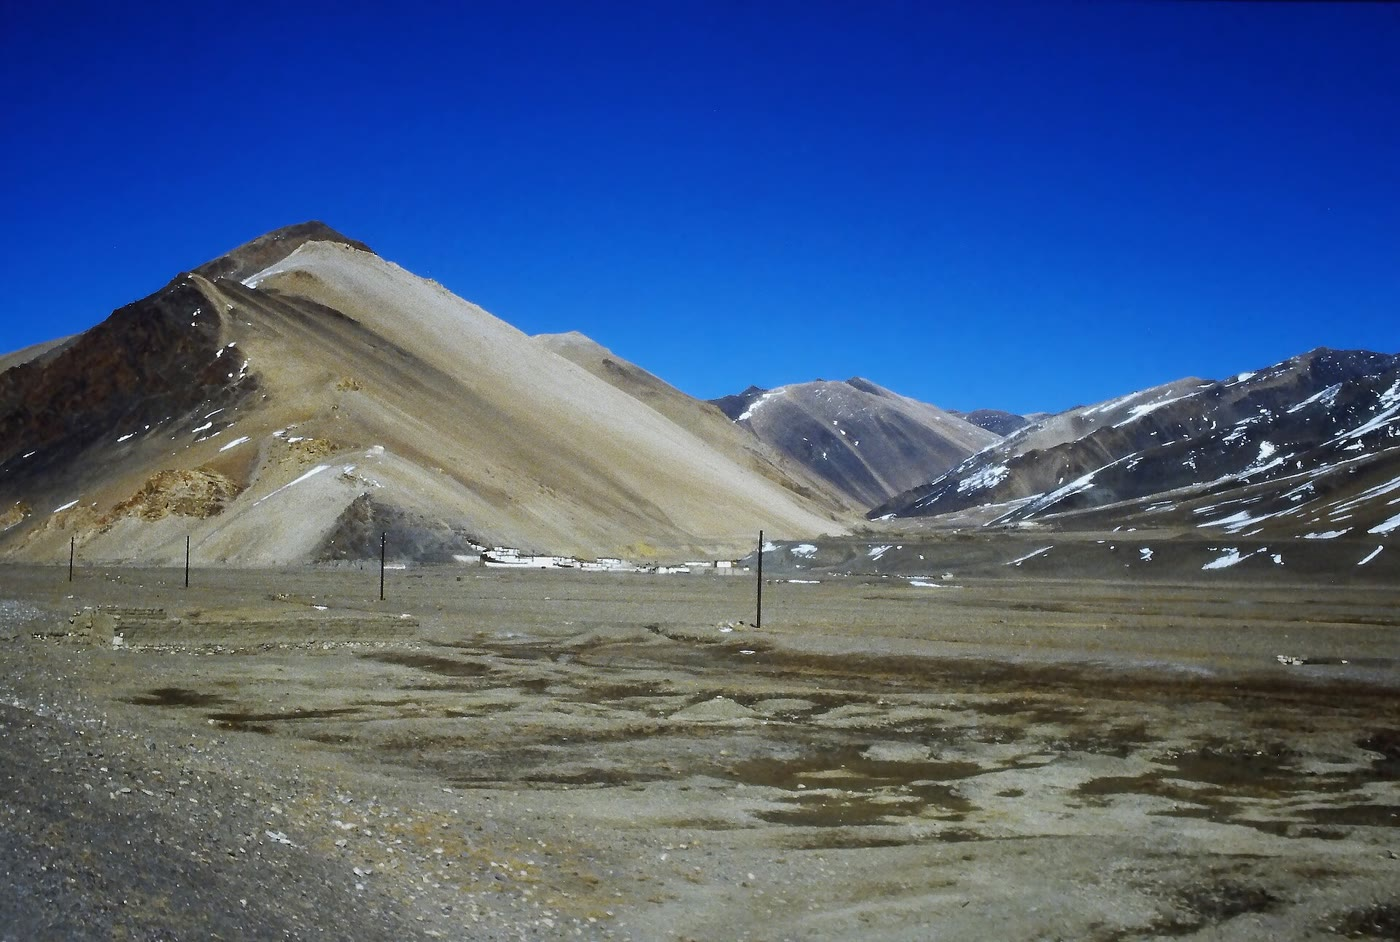
\includegraphics[width=0.66\linewidth]{images/book4/b2-14-tibet-plateau.jpg}
\par\smallskip{\small Het Tibetaans Plateau tussen Nepal en Shigatse: een vlakke bodem van grind en
schaars grasland, met een dorp, tussen kale bergen bedekt met puin, het geheel meer dan
vier kilometer boven zeeniveau.
Foto Jan Kranendonk, 1987, CC BY-SA 4.0.}
\end{omfigure}
% ledger: data:b4-etopo-tibet

\subsection{Het gewicht van een plateau}

Een plateau drukt op zijn omgeving. Op elke diepte tot aan de basis van zijn wortel staat een kolom
onder het plateau onder een hogere druk dan een kolom onder de laaglanden ernaast;
pas op de compensatiediepte zijn de twee gelijk. De hoge kolom duwt naar buiten.

\begin{proposition}[Overtollige potentiële energie van een plateau]\label{prop:b2:himalaya-andes:gpe}
Onder de hypothesen van \cref{prop:b2:himalaya-andes:airy}, met zwaartekrachtversnelling $g$, is de integraal van
de overtollige lithostatische druk van de plateaukolom ten opzichte van de normale kolom, van de top
van het plateau tot de compensatiediepte aan de basis van zijn wortel $r$, gelijk aan
\[
  \Delta F = \rho_c g h \left(H + \frac{h}{2} + \frac{r}{2}\right) .
\]
Het is de overtollige gravitationele potentiële energie van de plateaukolom per oppervlakte-eenheid, en de
kracht per lengte-eenheid van de rand van het plateau waarmee het plateau op zijn
omgeving duwt.
\end{proposition}

\begin{proof}
Meet de diepte $z$ naar beneden vanaf zeeniveau. In de plateaukolom is de druk $p_1 =
\rho_c g (z + h)$ van $z = -h$ tot $L = H + r$. In de normale kolom is ze nul boven
zeeniveau, $\rho_c g z$ in de korst, en $\rho_c g H + \rho_m g (z - H)$ daaronder. Het verschil $p_1
- p_0$ stijgt van 0 bij $z = -h$ tot $\rho_c g h$ op zeeniveau; het behoudt deze waarde door de
normale korst, waar beide kolommen korst zijn; onder $z = H$ neemt het lineair af, met
$(\rho_m - \rho_c) g$ per meter, en bereikt nul bij $L$ omdat $(\rho_m - \rho_c) r = \rho_c
h$. De integraal is de oppervlakte van dit trapezium: $\rho_c g h\,(h/2 + H + r/2)$. De arbeid die
de drukken verrichten wanneer de twee kolommen zijwaarts materiaal uitwisselen, is deze integraal; daarom
meet ze zowel de energie als de duw.
\end{proof}

\begin{omfigure}
\centering
% figdata/bachelor-2/plateaus.py part pressure (h = 4.8 km, H = 35 km, 2700 and 3300 kg/m3)
\begin{tikzpicture}
\begin{axis}[width=0.62\linewidth, height=5.6cm, y dir=reverse, xmin=0, xmax=160, ymin=-12,
  ymax=60, xlabel={overdruk $p_1 - p_0$ (\unit{MPa})}, ylabel={diepte onder zeeniveau
  (\unit{km})}, tick label style={font=\scriptsize}, label style={font=\small},
  xtick pos=bottom, ytick pos=left, clip=false]
\addplot[fill=omThm!20, draw=omThm, line width=1pt] table[x expr=\thisrow{p_high_MPa}-\thisrow{p_ref_MPa}, y=z_km] {figdata/out/bachelor-2-plateaus-pressure.dat} \closedcycle;
\draw[dashed] (axis cs:0,0) -- (axis cs:160,0);
\draw[dashed] (axis cs:0,35) -- (axis cs:160,35);
\draw[dashed] (axis cs:0,56.6) -- (axis cs:160,56.6);
\node[font=\scriptsize, anchor=north east] at (axis cs:160,0) {zeeniveau};
\node[font=\scriptsize, anchor=north east] at (axis cs:160,35) {normale Moho, $H$};
\node[font=\scriptsize, anchor=south east] at (axis cs:160,56.6) {basis van de wortel, $H + r$};
\node[font=\scriptsize, anchor=west] at (axis cs:100,-8.4) {top van het plateau, $-h$};
\node[font=\scriptsize, align=center] at (axis cs:60,20) {oppervlakte $= \Delta F$\\$\approx\qty{6.1e12}{N.m^{-1}}$};
\end{axis}
\end{tikzpicture}
\par\smallskip{\small De overtollige lithostatische druk van een plateaukolom ten opzichte van een normale
kolom, voor $h = \qty{4.8}{km}$, $H = \qty{35}{km}$ en dichtheden 2700 en
\qty{3300}{kg.m^{-3}}: ze stijgt door het plateau, blijft op $\rho_c g h = \qty{127}{MPa}$
door de normale korst, en daalt tot nul aan de basis van de wortel. De gearceerde oppervlakte is de
overtollige potentiële energie van \cref{prop:b2:himalaya-andes:gpe}.}
\end{omfigure}
% values (plateaus.py): tibet_gpe 6.12179e12 N/m for h = 4.8

Voor Tibet is $r = 4.5 \times 4.8 = \qty{21.6}{km}$ en $\Delta F = 2700 \times 9.8 \times 4800
\times (35000 + 2400 + 10800) \approx \qty{6.1e12}{N.m^{-1}}$. Verdeeld over een lithosfeer van
\qty{100}{km} dik is dat een gemiddelde overtollige spanning van ongeveer \qty{60}{MPa}, van de orde van de
spanningen die gesteenten breken. Een plateau dat zo zwaar is, kan niet meer gewoon rijzen: het neigt uit te vloeien.

\begin{definition}[Gravitationele ineenstorting]\label{def:b2:himalaya-andes:collapse}
De \emph{gravitationele ineenstorting}\index{gravitationele ineenstorting (van een orogeen)} van een \omterm{def:b2:alpine-orogen:orogen}{orogeen}
is het uitvloeien van zijn verdikte korst onder zijn eigen gewicht, door rek van de hoge
gebieden en uitwaartse stroming of overschuiving aan de randen, aangedreven door de overtollige potentiële energie van
de verdikte kolommen.
\end{definition}

Tibet wordt uitgerekt terwijl India er nog tegen duwt. Over Zuid-Tibet snijden
noord--zuid-riften het plateau en vangen ze oost--west-rek op: ongeveer $9 \pm \qty{2}{mm}$ per jaar in
totaal tussen \ang{81} en \ang{92}~OL, $1.3 \pm \qty{0.3}{mm}$ per jaar op de rift van Yadong--Gulu
alleen; ten noorden van Nepal tonen de GPS-stations dat het zuidelijke plateau uitrekt met ongeveer
\num{12e-9} per jaar. Aardbevingen vertellen hetzelfde verhaal: overschuivingen en \omterm{def:b2:himalaya-andes:thickening}{korstverdikking}
overheersen in het lagere terrein rond het plateau, horizontale verschuivingen en afschuivingen in het binnenste.
Waarom het uitrekt, staat ter discussie. In het oostelijke plateau is de rek gelezen als \omterm{def:b2:himalaya-andes:collapse}{gravitationele
ineenstorting}, aangedreven door het gewicht van het plateau; in het zuiden verbinden anderen ze met de gebogen vorm
van de Himalaya-boog, waarlangs de overschuivingen uiteenlopen, of met India dat eronder schuift.
% ledger: wang21:rifts, ader12:extension

\subsection{Zijwaarts ontsnappen}

\begin{definition}[Laterale extrusie]\label{def:b2:himalaya-andes:extrusion}
\emph{Laterale extrusie}\index{laterale extrusie} (ontsnappingstektoniek) is het zijwaarts uitdrijven van
blokken korst of lithosfeer uit een botsingszone, langs grote horizontale verschuivingen,
ongeveer loodrecht op de convergentierichting, naar een vrije grens.
\end{definition}

Ten oosten van Tibet wordt Azië niet alleen verkort; het wordt opzij geduwd. Lange linksdraaiende horizontale
verschuivingen, waaronder de breuken van de Rode Rivier en de Altyn Tagh, worden gelezen als geleiders van
de ontsnapping naar het oosten en zuidoosten van grote blokken, eerst het Sundablok van Zuidoost-Azië,
daarna Tibet en Zuid-China, terwijl aan hun verre uiteinden riften en jonge oceaanbekkens opengingen.
Experimenten waarbij een starre stempel in een laag plasticine werd gedrukt, gaven zulke breuken;
modellen die Azië als een doorlopende viskeuze plaat behandelden, gaven in plaats daarvan brede verdikking, zonder
grote breuken. GPS ondersteunt de beweging van blokken: ten opzichte van het stabiele Siberië beweegt het
Tarimbekken ruwweg naar het noorden met ongeveer \qty{14}{mm} per jaar en Zuid-China naar het oostzuidoosten
met ongeveer \qty{8}{mm} per jaar. Hoeveel van de opmars van India door verdikking is opgevangen en hoeveel
door extrusie, is nog omstreden.
% ledger: jiao23:extrusion

\section{De Andes}\label{sec:b2:himalaya-andes:andes}

De Nazcaplaat duikt onder Zuid-Amerika met ongeveer \qty{72}{mm} per jaar bij
\ang{20}~ZB, naar het oostnoordoosten, volgens de hoeksnelheden van NNR-MORVEL56. Er is geen continent
aangekomen, en toch dragen de Centrale Andes het op een na hoogste plateau op Aarde.
% ledger: nnr56:poles
% values (plateaus.py): v_nazca_southamerica 72.52 mm/yr, azimuth 74.5

Van west naar oost omvatten ze, tussen ongeveer \ang{15} en \ang{27}~ZB, vijf zones: de
\emph{voorboog}; de \emph{Westelijke Cordillera}, de vulkanische boog; het hoogplateau, de
\emph{Altiplano} in het noorden en de \emph{Puna} in het zuiden; de \emph{Oostelijke
Cordillera}; en de dunhuidige \omterm{def:b2:alpine-orogen:ftb}{plooi- en overschuivingsgordel} van de \emph{Subandiene zone}, die
overgaat in de Chacovlakte. Het profiel hierboven doorkruist ze op \ang{20}~ZB: vanaf de trog,
waarvan de diepste knoop \qty{7.7}{km} onder zeeniveau ligt op \ang{71.4}~WL, klimt het oppervlak
meer dan \qty{11}{km} over ongeveer \qty{240}{km} tot de rand van het plateau op \ang{69.1}~WL;
het plateau blijft boven \qty{3000}{m} over \qty{440}{km} met een
gemiddelde van \qty{3760}{m}. De gemiddelde hoogte is \qty{3.7}{km} in de Altiplano en \qty{4.4}{km} in
de Puna. Ten noorden van \ang{23}~ZB ligt de Moho meestal dieper dan \qty{60}{km}; onder de
centrale Altiplano is de korst 59 tot \qty{64}{km} dik.
% ledger: gerbault05:andes, gerbault05:moho, data:b4-etopo-andes

\begin{omfigure}
\centering
\begin{tikzpicture}[x=0.56cm, y=0.38cm, font=\scriptsize]
% mantle background
\fill[gray!12] (0,-2.6) -- (5,-3.6) -- (8,-5.6) -- (10,-9.1) -- (12,-12.6) -- (13.2,-14.6) -- (26,-14.6)
  -- (26,-4.5) -- (20,-4.7) -- (17.5,-6.0) -- (15,-7.3) -- (11,-7.0) -- (9.5,-6.2) -- (8,-4) -- (5,-2)
  -- (0,-1) -- cycle;
% ocean water
\fill[blue!8] (0,0) -- (6.33,0) -- (5,-2) -- (0,-1) -- cycle;
% Nazca slab
\fill[gray!45] (0,-1) -- (5,-2) -- (8,-4) -- (10,-7.5) -- (12,-11) -- (14,-14.5) -- (13.2,-14.6)
  -- (12,-12.6) -- (10,-9.1) -- (8,-5.6) -- (5,-3.6) -- (0,-2.6) -- cycle;
% South American crust
\fill[orange!22] (5,-2) -- (8,1) -- (9,1.9) -- (10.2,2.0) -- (11,2.0) -- (15,2.0) -- (15.6,2.6) -- (16.8,2.4)
  -- (17.5,1.6) -- (20,0.6) -- (20.6,0.4) -- (26,0.3) -- (26,-4.5) -- (20,-4.7) -- (17.5,-6.0) -- (15,-7.3)
  -- (11,-7.0) -- (9.5,-6.2) -- (8,-4) -- cycle;
% Altiplano basin fill
\fill[yellow!45] (11,2.0) -- (15,2.0) -- (14.6,1.0) -- (11.4,1.0) -- cycle;
% surface line
\draw[line width=0.5pt] (0,-1) -- (5,-2) -- (8,1) -- (9,1.9) -- (10.2,2.0) -- (11,2.0) -- (15,2.0) -- (15.6,2.6)
  -- (16.8,2.4) -- (17.5,1.6) -- (20,0.6) -- (20.6,0.4) -- (26,0.3);
% arc volcanoes
\fill[red!60!black] (8.8,1.75) -- (9.2,2.9) -- (9.6,1.95) -- cycle;
\fill[red!60!black] (9.8,1.95) -- (10.2,2.8) -- (10.6,2.0) -- cycle;
\draw[red!60!black, decorate, decoration={snake, amplitude=0.6pt, segment length=4pt}] (10.8,-8.0) -- (9.9,1.6);
% Subandean decollement and splays
\draw[thick] (16.0,-1.2) -- (20.55,0.42);
\draw (17.4,-0.7) -- (17.85,1.45);
\draw (18.4,-0.35) -- (18.8,1.08);
\draw (19.4,0.0) -- (19.7,0.72);
% Moho
\draw[dashed] (8,-4) -- (9.5,-6.2) -- (11,-7.0) -- (15,-7.3) -- (17.5,-6.0) -- (20,-4.7) -- (26,-4.5);
% labels
\node at (2.6,-0.5) {Stille Oceaan};
\node at (2.4,-2.2) {Nazcaplaat};
\draw[-{Latex[length=1.6mm]}] (1.6,-2.8) -- (3.2,-3.0);
\node[anchor=south] (tr) at (4.3,0.9) {trog};
\draw[->] (tr.south) -- (5,-1.8);
\node[anchor=south east] at (7.6,1.0) {voorboog};
\node[anchor=south, align=center] at (9.7,3.0) {Westelijke\\Cordillera (boog)};
\node[anchor=south] at (13,2.1) {Altiplano};
\node[anchor=south, align=center] at (16.4,2.7) {Oostelijke\\Cordillera};
\node[anchor=south west] at (18.6,1.3) {Subandien};
\node[anchor=south] at (23.5,0.4) {Chacovlakte};
\node at (13,-3.2) {dikke korst};
\node at (23.2,-2.0) {Braziliaans schild};
\node[anchor=north] at (23.2,-4.6) {Moho};
\node at (14.2,-9.6) {mantelwig};
\node at (21,-10) {mantel};
\node[rotate=-50] at (12.75,-12.9) {plaat};
\draw[-{Latex[length=2mm]}] (1.2,4.6) -- (0.2,4.6);
\node[anchor=south] at (0.7,4.6) {W};
\draw[-{Latex[length=2mm]}] (24.8,4.6) -- (25.8,4.6);
\node[anchor=south] at (25.3,4.6) {O};
\end{tikzpicture}
\par\smallskip{\small Een schematische doorsnede door de Centrale Andes bij \ang{20}~ZB (niet op
schaal). De Nazcaplaat zinkt onder de voorboog; \omterm{def:b2:magma-emplacement:magma}{magma} stijgt op uit de mantelwig (golvende
lijn) naar de boog van de Westelijke Cordillera; de Altiplano, met zijn dikke bekkenvulling, ligt
tussen de twee cordillera's, boven een korst van ongeveer \qty{60}{km} dik; de dunhuidige
Subandiene gordel is naar het oosten over het Braziliaanse schild geschoven.}
\end{omfigure}
% ledger: gerbault05:andes, gerbault05:moho

\subsection{Hoe de korst dik werd}

Waar kwam de extra korst van de Altiplano vandaan? De eerste kandidaat is verkorting:
druk een strook korst samen en ze wordt dikker, met behoud van haar doorsnede-oppervlakte.

\begin{proposition}[Verdikking door verkorting]\label{prop:b2:himalaya-andes:shortening}
Laat een korst met uniforme dikte $H$ worden verkort, zonder winst of verlies van gesteente, tot een korst
met dikte $T$ over een breedte $W$, waarbij de doorsnede evenwijdig aan de verkorting blijft. Haar
oorspronkelijke breedte was $W_0 = W T/H$, en de verkorting is
\[
  S = W_0 - W = W\,\frac{T - H}{H} .
\]
\end{proposition}

\begin{proof}
De doorsnede-oppervlakte van de korst blijft behouden, zoals in de oppervlaktebalans van
\cref{prop:b2:alpine-orogen:balance}: $W_0 H = W T$. Dus $W_0 = WT/H$ en $S = W_0 - W =
W(T - H)/H$.
\end{proof}

Op \ang{20}~ZB is het plateau ongeveer \qty{440}{km} breed; als zijn korst, ongeveer \qty{60}{km} dik,
ooit \qty{35}{km} was, is de benodigde verkorting $440 \times 25/35 \approx \qty{314}{km}$.
\omterm{def:b2:alpine-orogen:balanced}{Gebalanceerde doorsneden} bij 16--\ang{21}~ZB vinden ongeveer \qty{50}{km} verkorting in de Altiplano
en meer dan \qty{200}{km} in de Subandiene zone sinds het Oligoceen. De korstvolumes
die uit de verkorting worden berekend, liggen ongeveer \qty{20}{\percent} onder die welke uit de diepte
van de Moho worden berekend. Een deel van het verschil kan aan verkeerde aannamen liggen, over de begindikte of
de aard van de seismische Moho; een deel kan korst zijn die op andere manieren is toegevoegd. Eén compilatie bij
\ang{21}~ZB schrijft minstens \qty{55}{\percent} van de wortel toe aan tektonische verkorting, tot
\qty{20}{\percent} aan de hydratatie van de mantelwig van de voorboog, en slechts ongeveer \qty{5}{\percent} aan magmatische toevoeging en
tektonische erosie. Gesteente kan ook binnen de gordel bewegen:
verschillen in korstdikte scheppen verschillen in potentiële energie, zoals in Tibet, en
die kunnen de hete onderkorst van dik naar dun doen vloeien.
% ledger: gerbault05:andes, gerbault05:volume, gerbault05:moho, data:b4-etopo-andes

\begin{omfigure}
\centering
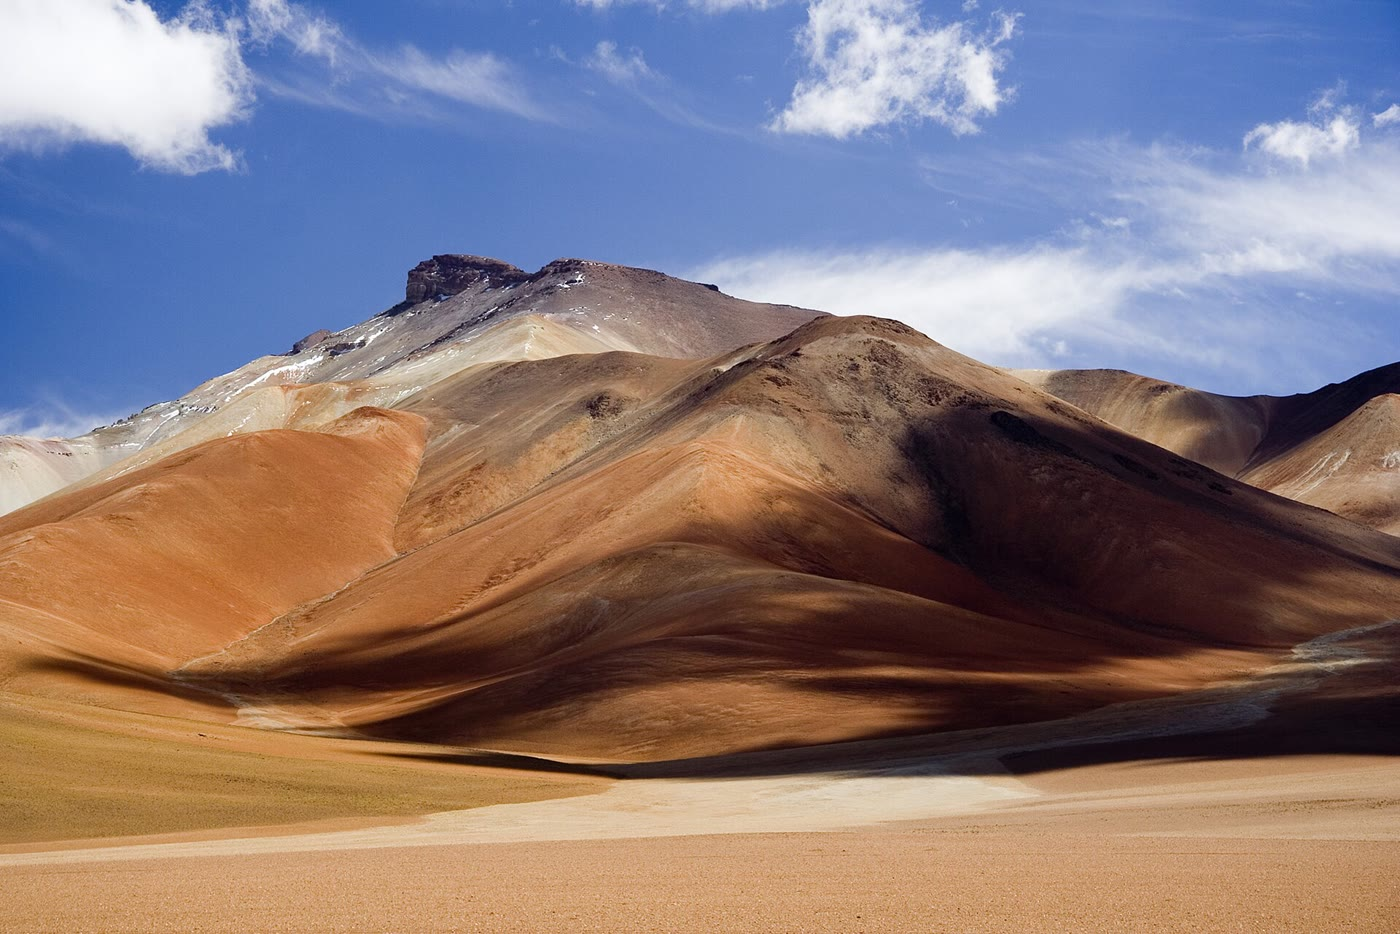
\includegraphics[width=0.66\linewidth]{images/book4/b2-14-altiplano.jpg}
\par\smallskip{\small De Boliviaanse Altiplano: een vlakte van zand en grind aan de voet van
kale heuvels die door hun gesteenten rood, oker en grijs zijn gekleurd. Foto Luca Galuzzi, 2006, CC BY-SA 2.5.}
\end{omfigure}
% ledger: gerbault05:andes

\subsection{Vlakke platen en verloren wortels}

De hoek van de plaat ligt niet vast, en dat doet ertoe aan het oppervlak.

\begin{definition}[Subductie met vlakke plaat]\label{def:b2:himalaya-andes:flat-slab}
\emph{Subductie met vlakke plaat}\index{subductie met vlakke plaat} is subductie waarbij de plaat,
na haar eerste afdaling, over honderden kilometers bijna horizontaal onder de bovenliggende plaat loopt
voordat ze weer wegzinkt.
\end{definition}

Langs de Andes zijn vandaag twee segmenten van de Nazcaplaat vlak, het Peruaanse segment, vlak
sinds ongeveer \qty{15}{Ma}, en het Pampeaanse segment, sinds ongeveer \qty{18}{Ma}. Erboven zijn er
geen actieve vulkanen. Toen de Pampeaanse plaat vlakker werd, verschoof de boog landinwaarts en spuwde
minder lava; boven de vlakke segmenten is hij stilgevallen. De afstand tussen boog en trog uit Boek~3
verklaart de verschuiving landinwaarts: hoe flauwer de plaat onder de boog, hoe verder van de trog ze
de diepte bereikt waarop de wig smelt; en een plaat die boven die diepte vlak blijft, laat
helemaal geen hete mantelwig over om te smelten.
% ledger: gauthier24:flat

\begin{definition}[Lithosferische delaminatie]\label{def:b2:himalaya-andes:delamination}
\emph{Lithosferische delaminatie}\index{lithosferische delaminatie} is het loskomen en
wegzinken in de asthenosfeer van het onderste deel van een verdikte lithosfeer, zijn
mantellithosfeer en soms een dichte onderkorst, vervangen door hete asthenosfeer.
\end{definition}

Delaminatie is voorgesteld onder de zuidelijke Puna, tussen \ang{24} en \ang{27}~ZB,
ongeveer 2 tot \qty{3}{Ma} geleden, waar jonge mafische lava's uitvloeiden; en langs het plateau zijn veranderingen
van korstdikte en hoogte verbonden met een mantellithosfeer die al verdwenen is
onder de zuidelijke Altiplano en nog niet volledig onder de centrale Altiplano. Het verlies van een
dicht manteldeksel maakt de overblijvende kolom lichter: het oppervlak rijst zonder verdere
verkorting. De Puna ligt ongeveer \qty{1}{km} hoger dan de Altiplano op een korst die ongeveer
\qty{11}{km} dunner is, een contrast dat ofwel een lichtere Puna-korst ofwel een lichtere mantel
eronder vraagt.
% ledger: gerbault05:delamination, gerbault05:moho

\section{Twee gordels vergeleken}\label{sec:b2:himalaya-andes:compared}

De twee plateaus lijken van ver op elkaar en verschillen in bijna al het andere, zoals de tabel
hieronder samenvat.

\begin{omfigure}
\centering\small
\begin{tabular}{>{\raggedright\arraybackslash}p{0.2\linewidth}|>{\raggedright\arraybackslash}p{0.34\linewidth}|>{\raggedright\arraybackslash}p{0.34\linewidth}}
 & Himalaya en Tibet & Centrale Andes \\ \hline
motor & continent tegen continent nadat de oceaan sloot & oceanische plaat die onder een continent zinkt \\
as & sutuur met \omterm{def:b2:alpine-orogen:ophiolite}{ofiolieten} & vulkanische boog boven de plaat \\
magmatisme & korstsmelten: \omterm{def:b2:crustal-melting:leucogranite}{leucogranieten} & boogandesieten; mafische lava's waar de lithosfeer verloren ging \\
convergentie & ongeveer \qty{45}{mm} per jaar, de helft opgevangen in de keten & ongeveer \qty{72}{mm} per jaar, grotendeels verbruikt door subductie \\
grote aardbevingen & op de MHT, Assam 1950, $M_w \approx 8.5$ & op het subductievlak, Chili 1960, $M_w$ 9.5 \\
plateau & gemiddeld \qty{4.8}{km} over \qty{1180}{km}; korst 70--\qty{75}{km} & gemiddeld \qty{3.8}{km} over \qty{440}{km}; korst ongeveer \qty{60}{km} \\
plateautektoniek & oost--west-rek, extrusie & verkorting op de flanken; delaminatie voorgesteld \\
voorland & Indo-Gangetische voordiepte en Siwalikmolasse & Subandiene gordel en Chacovlakte \\
\end{tabular}
\par\smallskip{\small De twee gordels naast elkaar; de bronnen worden in de paragrafen hierboven geciteerd,
en de aardbeving van Chili is de grootste die sinds 1900 is geregistreerd.}
\end{omfigure}
% ledger: lave00:setting, lave00:siwaliks, weinberg16:himalaya, ader12:mht, ader12:quakes, usgs:largest, gerbault05:andes, gerbault05:moho, gerbault05:delamination, nnr56:poles, data:b4-etopo-tibet, data:b4-etopo-andes, cattin01:crust, wang21:rifts, jiao23:extrusion

Het diepste verschil zit in wat er naar beneden gaat. In de Andes blijft de oceanische plaat zinken, en
het grootste deel van de convergentie, ongeveer \qty{72}{mm} per jaar, wordt aan de trog verbruikt; de
bovenplaat over zo'n 30 miljoen jaar met \qty{310}{km} verkorten, zou er maar ongeveer \qty{10}{mm} per
jaar van vragen. In de Himalaya kan niets lichts lang zinken, zodat de convergentie wordt besteed aan
stapelen, verdikken en Azië opzij duwen. Beide gordels laten plateaus groeien omdat een dikke korst
een hoge korst is; beide plateaus stoppen met rijzen wanneer hun eigen gewicht de duw aan hun
randen in evenwicht houdt, en dan vloeien ze uit.
% ledger: nnr56:poles, gerbault05:andes, ader12:mht, jiao23:extrusion

\section{Hoe hoog kan een berg zijn?}\label{sec:b2:himalaya-andes:heights}

De hoogste top, de Everest, staat \qty{8848.86}{m} boven zeeniveau volgens de gezamenlijke meting
die in 2020 werd bekendgemaakt. Waarom geen twintig kilometer? Een ruwe grens komt van de sterkte van gesteente.

\begin{proposition}[Een hoogtegrens uit de sterkte van gesteente]\label{prop:b2:himalaya-andes:height}
Een gesteentekolom met dichtheid $\rho$ die een hoogte $h$ boven haar omgeving uitsteekt, zonder
zijdelingse steun boven het niveau van die omgeving, draagt aan haar voet een verticale spanning $\rho g h$ en een
horizontale spanning nul op haar vrije zijden, dus een spanningsverschil $\rho g h$. Als het
gesteente bezwijkt bij het spanningsverschil $\sigma_d$, blijft de kolom alleen staan als $h < \sigma_d/(\rho
g)$.
\end{proposition}

\begin{proof}
Aan de voet van de kolom is de verticale spanning het gewicht van het gesteente erboven per oppervlakte-eenheid,
$\rho g h$. De zijden zijn vrij, dus de horizontale spanning is daar nul. Het
spanningsverschil is het verschil tussen de grootste en de kleinste hoofdspanning, hier $\rho g h - 0$.
Bezwijken wordt alleen vermeden als het onder $\sigma_d$ blijft.
\end{proof}

Een echte berg heeft hellende flanken die zijn kern insluiten, zodat de spanning eronder
kleiner is; neem als orde van grootte de helft, $\rho g h/2$. Voor de Everest is $2700 \times 9.8
\times 8849/2 \approx \qty{117}{MPa}$. De wet van Byerlee uit Boek~3 stelt de
wrijvingssterkte van gesteente op een breuk onder een normaalspanning van \qty{200}{MPa} op $50 + 0.6 \times 200 =
\qty{170}{MPa}$: dezelfde orde. Een berg die drie keer hoger is, zou zijn basis ver voorbij
wat gesteente kan dragen belasten; hij zou bezwijken en uitvloeien. Op Aarde liggen toppen van acht tot negen kilometer
dicht bij de grens, en een plateau, dat lang voordat zijn toppen bezwijken uitvloeit, vlakt af
op vijf.
% ledger: tht:everest, byerlee:1975

\section*{Oefeningen}\label{sec:b2:himalaya-andes:exercises}

Gegevens voor de oefeningen: $g = \qty{9.8}{m.s^{-2}}$; dichtheden van korst en mantel
\qty{2700}{kg.m^{-3}} en \qty{3300}{kg.m^{-3}}, tenzij anders vermeld; normale korst $H =
\qty{35}{km}$.

\begin{exercise}[$\star$]\label{exo:b2:himalaya-andes:1}
Een plateau ligt op een gemiddelde hoogte van \qty{3.0}{km}. Bereken met
\cref{prop:b2:himalaya-andes:airy} (a) zijn Airy-wortel, (b) zijn korstdikte.
(c) Met hoeveel zou \qty{10}{km} extra korst het opheffen?
\end{exercise}

\begin{exercise}[$\star$]\label{exo:b2:himalaya-andes:2}
Een doorsnede door de Himalaya van Nepal loopt van de Gangesvlakte tot het Tibetaans Plateau.
(a) Som in volgorde de eenheden op die ze doorkruist en de breuken die ze scheiden. (b) Welke breuk
is een afschuiving? (c) Hoe verandert de metamorfe graad naar het noorden tot aan de
Hoge-Himalayareeks, en daarboven?
\end{exercise}

\begin{exercise}[$\star$]\label{exo:b2:himalaya-andes:3}
In Midden-Nepal is een rivierterras dat \qty{9.2}{kyr} geleden werd verlaten, met
\qty{196.5}{m} verkort over de plooien van de Frontale Hoofdoverschuiving. (a) Bereken de gemiddelde
verkortingssnelheid in millimeter per jaar. (b) Vergelijk ze met de GPS-convergentie over de keten,
\qty{17.8}{mm} per jaar. (c) Wat zegt de overeenstemming over de breuken ten noorden van de MFT?
\end{exercise}

\begin{exercise}[$\star$]\label{exo:b2:himalaya-andes:4}
Deel elke waarneming in bij \omterm{def:b2:himalaya-andes:types}{botsingsorogeen}, \omterm{def:b2:himalaya-andes:types}{orogeen van Andestype} of beide: (a) een sutuur bezet
met \omterm{def:b2:alpine-orogen:ophiolite}{ofiolieten}; (b) een rij actieve andesietvulkanen; (c) \omterm{def:b2:crustal-melting:leucogranite}{leucogranieten} die uit de
korst zijn gesmolten; (d) een diepe oceanische trog langs het front; (e) een \omterm{def:b2:alpine-orogen:foreland}{voorlandbekken} met \omterm{def:b2:alpine-orogen:foreland}{molasse};
(f) grote aardbevingen op een zacht hellende breuk onder de keten.
\end{exercise}

\begin{exercise}[$\star\star$]\label{exo:b2:himalaya-andes:5}
India beweegt met \qty{45}{mm} per jaar ten opzichte van Eurazië over de Himalaya; over Nepal
vangt de keten zelf \qty{17.8}{mm} per jaar op in het oosten en \qty{20.5}{mm} per jaar in het westen.
(a) Welke fractie van de convergentie neemt de keten in elk geval op? (b) Waar gaat de
rest heen? (c) Hoeveel verkorting vertegenwoordigt de rest over \qty{10}{Myr}?
\end{exercise}

\begin{exercise}[$\star\star$]\label{exo:b2:himalaya-andes:6}
(a) Bereken met \cref{prop:b2:himalaya-andes:gpe} de overtollige potentiële energie van de
Altiplano, gemiddelde hoogte \qty{3.7}{km}. (b) Vergelijk ze met die van Tibet op \qty{4.8}{km}.
(c) Toon aan dat voor een dun plateau, $h \ll H$, $\Delta F$ evenredig met $h$ groeit, en voor een
dik plateau sneller: wat betekent dat voor de groei van een plateau?
\end{exercise}

\begin{exercise}[$\star\star$]\label{exo:b2:himalaya-andes:7}
(a) Bereken $\rho g h/2$ onder de Everest, \qty{8848.86}{m} hoog, met $\rho =
\qty{2700}{kg.m^{-3}}$. (b) Volgens de wet van Byerlee is $\tau = 0.85\,\sigma_n$ onder \qty{200}{MPa}
normaalspanning en $\tau = \qty{50}{MPa} + 0.6\,\sigma_n$ daarboven; bereken $\tau$ voor $\sigma_n =
100$ en \qty{200}{MPa}. (c) Welke hoogte zou een sterkte van \qty{170}{MPa} toelaten, volgens dezelfde
vuistregel voor de orde van grootte?
\end{exercise}

\begin{exercise}[$\star\star$]\label{exo:b2:himalaya-andes:8}
De riften van Zuid-Tibet vangen $9 \pm \qty{2}{mm}$ per jaar oost--west-rek op tussen
\ang{81} en \ang{92}~OL. (a) Hoe breed is dat stuk op \ang{30}~NB, met \qty{111.19}{km} per
graad op een meridiaan? (b) Bereken de gemiddelde reksnelheid, per jaar en per seconde,
met haar bereik. (c) Vergelijk met de $(12.4 \pm 4.7) \times 10^{-9}$ per jaar die uit GPS ten noorden van Nepal is gevonden.
\end{exercise}

\begin{exercise}[$\star\star$]\label{exo:b2:himalaya-andes:9}
De vergrendelde Hoofdoverschuiving van de Himalaya onder Nepal bouwt een momenttekort op van
\qty{6.6e19}{N.m} per jaar; de aardbevingen van de laatste 500 jaar maakten slechts
\qty{0.9e19}{N.m} per jaar vrij. (a) Welke fractie van het tekort maakten ze vrij? (b) Bereken met $M_0 =
10^{1.5 M_w + 9.1}$\,\unit{N.m} het moment van een aardbeving met $M_w$ 8.5. (c) Hoe vaak
zouden zulke aardbevingen nodig zijn om het tekort te compenseren?
\end{exercise}

\begin{exercise}[$\star\star\star$]\label{exo:b2:himalaya-andes:10}
De Puna ligt \qty{0.7}{km} hoger dan de Altiplano (4.4 tegen \qty{3.7}{km}) op een korst die
\qty{11}{km} dunner is. Neem de korst van de Altiplano \qty{61.5}{km} dik en met dichtheid
\qty{2800}{kg.m^{-3}}, en een mantel van \qty{3300}{kg.m^{-3}} onder beide. (a) Schrijf de
gelijkheid van de massa's van de twee kolommen boven een gemeenschappelijke compensatiediepte. (b) Bepaal de
dichtheid die de korst van de Puna moet hebben als de korst alleen het verschil compenseert. (c) Vergelijk
met de opgegeven 150 tot \qty{200}{kg.m^{-3}}, en zeg wat het contrast anders zou kunnen verklaren.
\end{exercise}

\begin{exercise}[$\star\star\star$]\label{exo:b2:himalaya-andes:11}
Het vulkanische front staat waar de bovenkant van de plaat \qty{105}{km} diep ligt. (a) Bereken voor een plaat
die uniform onder \ang{30} helt, de afstand tussen boog en trog met de formule uit
Boek~3. (b) De plaat helt nu onder \ang{30} tot \qty{90}{km}, daarna onder slechts \ang{4}: bereken
de nieuwe afstand en de verschuiving van de boog landinwaarts. (c) Wat gebeurt er met de boog als de plaat vlak wordt
op \qty{95}{km} diepte en daar over \qty{300}{km} blijft?
\end{exercise}

\begin{exercise}[$\star\star\star$]\label{exo:b2:himalaya-andes:12}
Erosie verwijdert ongeveer \qty{300}{km^3} gesteente per kilometer Himalaya per miljoen jaar.
India voert korst aan van \qty{37.5}{km} dik met \qty{21}{mm} per jaar. (a) Hoeveel korst per
kilometer keten per miljoen jaar komt de gordel binnen? (b) Welke fractie verwijdert de erosie?
(c) Waar kan de rest zijn?
\end{exercise}

\begin{problem}[{Weekendprobleem --- twee plateaus}]\label{pb:b2:himalaya-andes:1}
De profielen over stroken in dit hoofdstuk geven de gemiddelde hoogte van de knopen over Tibet
(\qtyrange{86}{90}{\degree} OL) en over de Centrale Andes (\qtyrange{19}{21}{\degree} ZB).
Bemonsterd om de \ang{1.5} breedtegraad en om de graad lengtegraad, afgerond op \qty{10}{m}, luiden ze
als volgt. Tenzij anders vermeld zijn $g = \qty{9.8}{m.s^{-2}}$, $\rho_c = \qty{2700}{kg.m^{-3}}$,
$\rho_m = \qty{3300}{kg.m^{-3}}$ en is de normale korst $H = \qty{35}{km}$ dik.

\smallskip
\begin{center}\small
\begin{tabular}{l|ccccccccc}
breedtegraad (\unit{\degree} NB) & 26.5 & 28.0 & 29.5 & 31.0 & 32.5 & 34.0 & 35.5 & 37.0 & 38.5 \\ \hline
gemiddelde hoogte (\unit{m}) & 70 & 5000 & 5030 & 4830 & 5020 & 5150 & 5050 & 4470 & 2210
\end{tabular}

\smallskip
\begin{tabular}{l|cccccccc}
lengtegraad (\unit{\degree}) & $-71$ & $-70$ & $-69$ & $-68$ & $-67$ & $-66$ & $-65$ & $-64$ \\ \hline
gemiddelde hoogte (\unit{m}) & $-3310$ & 970 & 4150 & 3720 & 3740 & 4010 & 3030 & 1170
\end{tabular}
\end{center}
\smallskip

\noindent\textbf{Deel I --- De profielen lezen.}
\begin{enumerate}
\item Neem als plateau de monsters boven \qty{3000}{m} en bereken de gemiddelde hoogte van Tibet
$h_T$, afgerond op \qty{0.1}{km}.
\item Doe hetzelfde voor de Altiplano, $h_A$, en vergelijk met de gemiddelde hoogte van
\qty{3.7}{km} die voor de Altiplano en \qty{4.4}{km} die voor de Puna wordt opgegeven.
\item Hoe breed is elk plateau minstens, volgens de monsters (\qty{111.19}{km} per
graad breedtegraad; \qty{104.5}{km} per graad lengtegraad op \ang{20}~ZB)?
\item Bereken de gemiddelde helling van het Himalayafront tussen \ang{26.5} en \ang{28.0}~NB, als
percentage.
\item Waarom is het Andesprofiel zoveel asymmetrischer dan het Tibetaanse?
\end{enumerate}

\noindent\textbf{Deel II --- Airy-diktes.}
\begin{enumerate}[resume]
\item Bereken de Airy-wortel en de korstdikte $T_T$ van Tibet uit $h_T$.
\item Doe hetzelfde voor de Altiplano, $T_A$.
\item Vergelijk met de seismische diktes, 70 tot \qty{75}{km} onder Tibet en 59 tot
\qty{64}{km} onder de centrale Altiplano. Welke schatting zit er verder naast?
\item Welke korstdichtheid zou de Airy-dikte van Tibet gelijk maken aan \qty{72.5}{km}?
\item Welke dichtheid zou \qty{61.5}{km} geven voor de Altiplano?
\item Noem twee redenen, naast de korstdichtheid, waarom een lokale Airy-berekening de
waargenomen wortel kan missen.
\item De korst is \qty{37.5}{km} dik onder India en \qty{72.5}{km} onder Tibet. Schat met een
dichtheidscontrast aan de Moho van \qty{370}{kg.m^{-3}} en met de Bouguer-plaat, $\Delta g
= 2\pi G\,\Delta\rho\,t$, de Bouguer-anomalie van de wortel van Tibet ten opzichte van India, waarbij $t$ de
extra dikte onder zeeniveau is ($G = \qty{6.674e-11}{m^3.kg^{-1}.s^{-2}}$). Vergelijk met het
waargenomen verschil van \qty{460}{mGal}.
\end{enumerate}

\noindent\textbf{Deel III --- De Altiplano verkorten.} Op \ang{20}~ZB is het plateau
\qty{440}{km} breed en zijn korst ongeveer \qty{60}{km} dik.
\begin{enumerate}[resume]
\item Bereken met \cref{prop:b2:himalaya-andes:shortening} de herstelde breedte en de
benodigde verkorting als de korst vroeger \qty{35}{km} dik was.
\item \omterm{def:b2:alpine-orogen:balanced}{Gebalanceerde doorsneden} geven ongeveer \qty{50}{km} verkorting in de Altiplano en
\qty{200}{km} in de Subandiene zone. Welke fractie van de benodigde verkorting ontbreekt?
\item Als verkorting slechts \qty{55}{\percent} van de extra korst maakte, hoeveel verkorting is er dan
nodig?
\item De Subandiene gordel is dunhuidig. Waarom moet zijn verkorting toch ergens de korst
verdikken?
\item Veronderstel dat de \qty{314}{km} van Deel III over \qty{30}{Myr} is opgebouwd. Bereken de gemiddelde
snelheid, en de fractie van de huidige convergentie tussen Nazca en Zuid-Amerika, \qty{72}{mm} per jaar, die
ze vertegenwoordigt.
\item Waar gaat de rest van de convergentie heen?
\end{enumerate}

\noindent\textbf{Deel IV --- Het gewicht van Tibet.}
\begin{enumerate}[resume]
\item Bereken met \cref{prop:b2:himalaya-andes:gpe} en $h_T$ de overtollige potentiële
energie van Tibet per oppervlakte-eenheid.
\item Bereken ze voor de Altiplano met $h_A$, en de verhouding van de twee.
\item Verdeel de $\Delta F$ van Tibet over een lithosfeer van \qty{100}{km} dik: welke gemiddelde spanning
vertegenwoordigt ze?
\item De rek van Zuid-Tibet, \qty{9}{mm} per jaar over \qty{1060}{km}, komt overeen met hoeveel
vervorming per jaar?
\item Waarom kan Tibet oost--west uitrekken terwijl India het nog naar het noorden duwt?
\item Samengevat: geef de korstdikte van Tibet berekend uit zijn gemiddelde hoogte, afgerond
op de kilometer, en de fractie van de seismische \qty{72.5}{km} die ze verklaart.
\end{enumerate}
\end{problem}
